\begin{figure}[htbp]
\centering
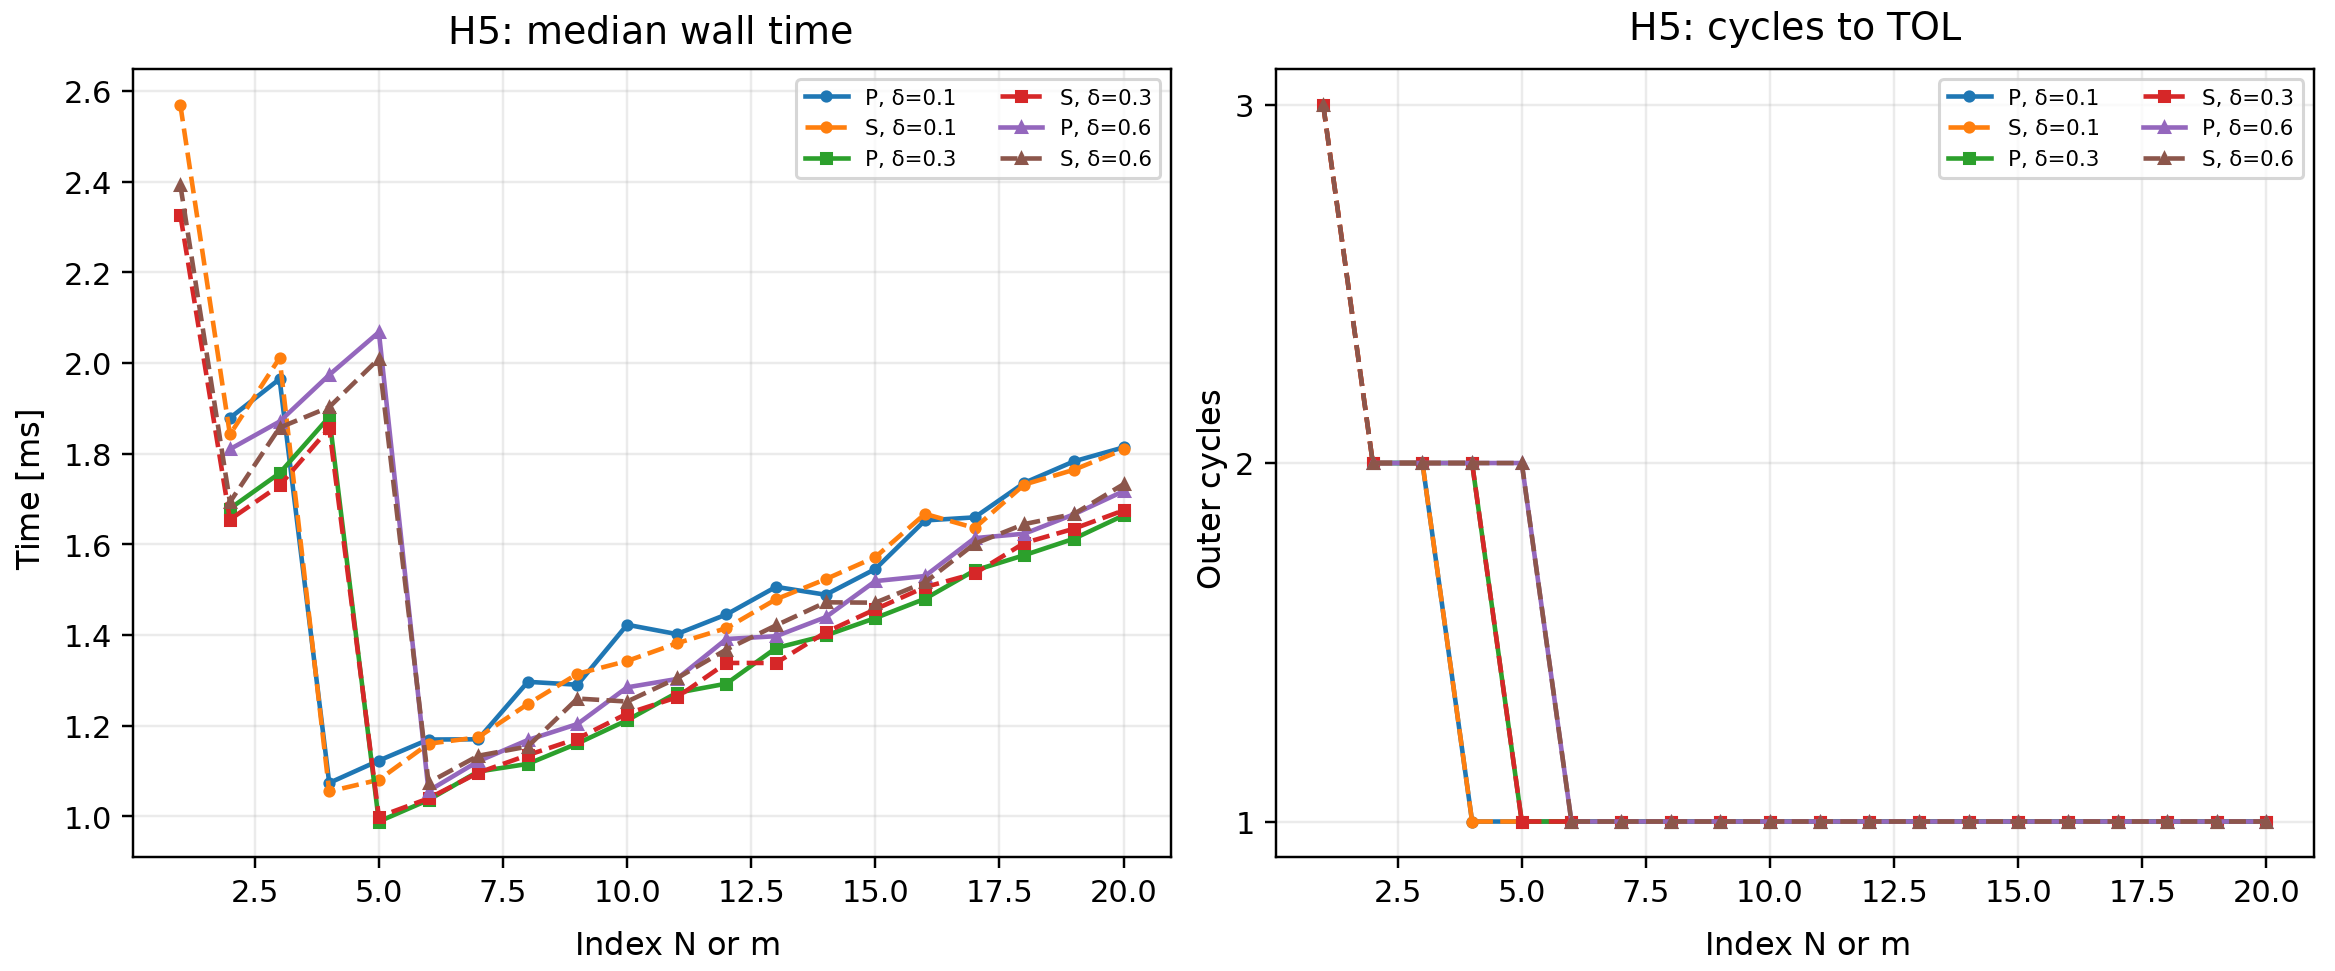
\includegraphics[width=0.96\textwidth]{figures/H5_time_cycles.png}
\caption{Complete sweep in $H_5$ for three initial distances. Left: median elapsed wall time. Right: number of outer cycles required to reach $\mathrm{TOL}=10^{-12}$. The first cycle of $P_N$ and $S_N$ has the same resources. With more than one cycle, memory is active, but that activation does not imply a resolved timing separation; the curves are interpreted together with the IQRs in this supplement.}
\label{fig:H5-practical-sweep}
\end{figure}
